\newpage
\thispagestyle{empty}
\mbox{}

\chapter{Resultados experimentales}
\label{ch:chapter3}

Al ya conocer como funciona el sistema en su totalidad se estudiarán diversos comportamientos que irán apareciendo en función de variar cada uno de sus parámetros. Para ello, el sistema completo se va a desplazar sobre un plano definido mediante una función gaussiana cuya base se sustenta en la figura \ref{FunGauss} y en la ecuación \ref{Funcion_Gaussiana}. 

Para los primeros 4 casos se particulariza la simulación del sistema en base a los siguientes datos: el centro se situé en $c_{o}=[0,0]$, el ángulo $\theta$ nulo, una desviación uniforme en ambos ejes $\sigma_{x}=\sigma_{y}=\frac{1}{1000}$ para que la matriz quede definida como $S = \bigl[\begin{smallmatrix}\frac{1000}{\sqrt{2}} & 0\\ 0 & \frac{1000}{\sqrt{2}}\end{smallmatrix}\bigr]$  y cuyo volumen es $p = 1$.

En primer lugar, se evalúa una situación inicial con N = 4, D = 30 y $\epsilon$=20 \footnote[8]{Recordar que este valor era la constante multiplicativa en \ref{GA}}. Este caso se va a usar como punto comparativo con el resto que se irán planteando a lo largo del capítulo. Se reflejará el camino siguiendo al gradiente estimado en comparación con el camino siguiendo el gradiente real, la evolución de cada componente del gradiente hasta llegar al punto máximo y finalmente una curva de error que posteriormente se definirá.

\begin{figure}[htb]
\centering
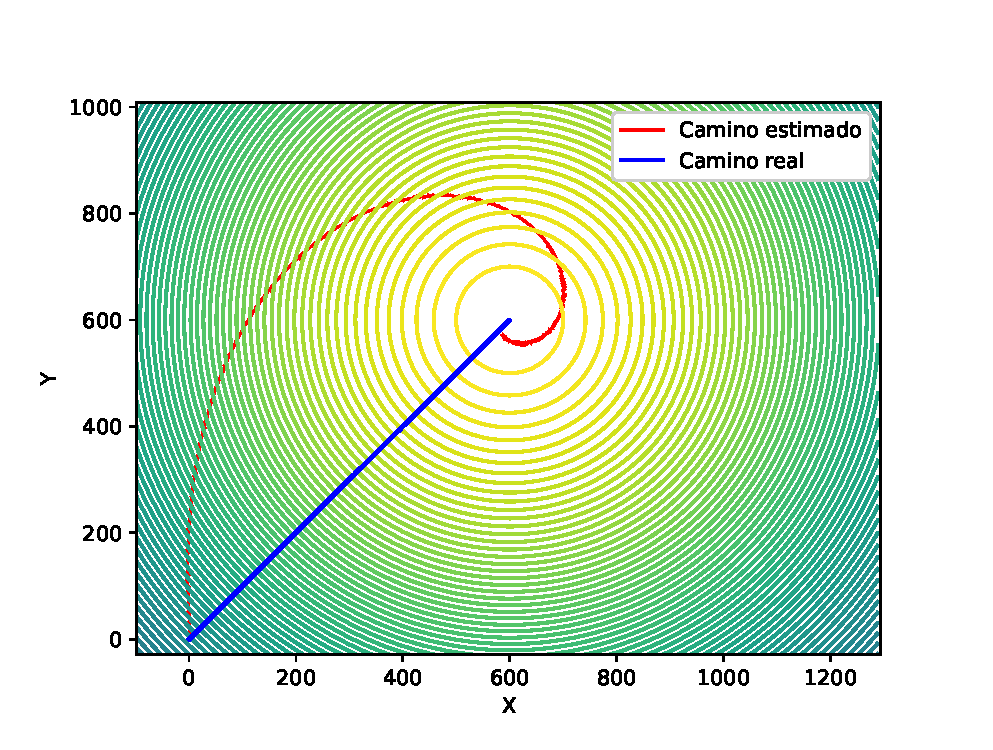
\includegraphics[width=0.75\textwidth]{figures/Caso_Inicial/Caminos.eps}
\caption{Comparativa entre el camino descrito por el gradiente y por el gradiente estimado.} \label{Dif_Caminos}
\end{figure}

\begin{figure}[H]
\centering
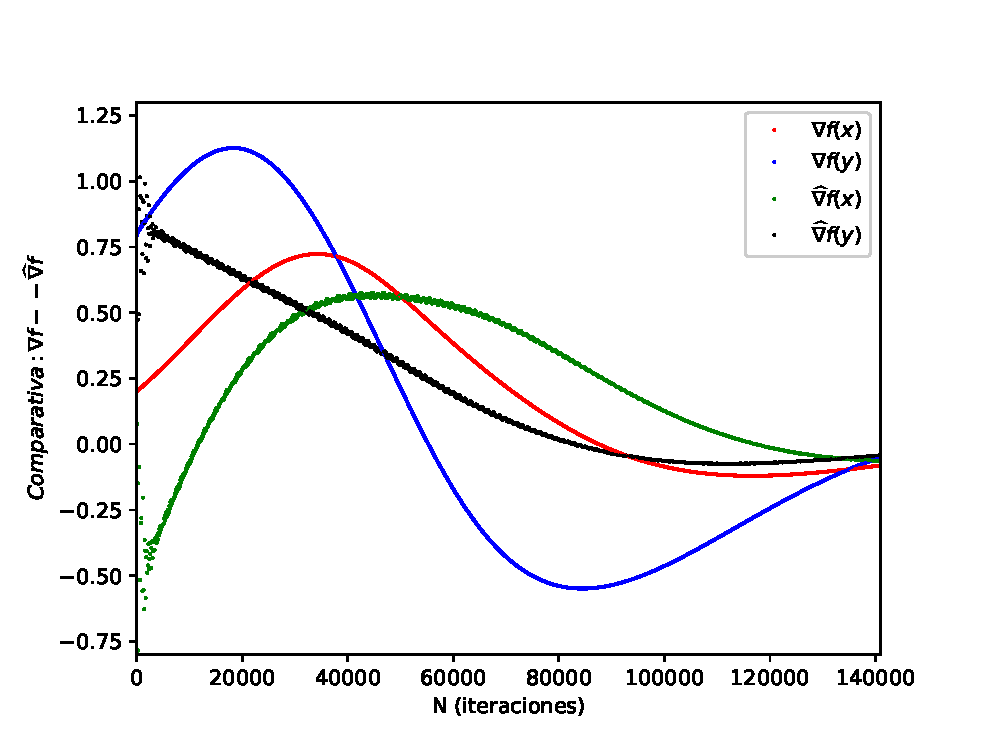
\includegraphics[width=0.75\textwidth]{figures/Graficas_Nuevas/Caso_Inicial/Figure_3.eps}
\caption{Comparativa de las componentes del gradiente entre el real y el estimado.} \label{grad}
\end{figure}

\begin{figure}[H]
\centering
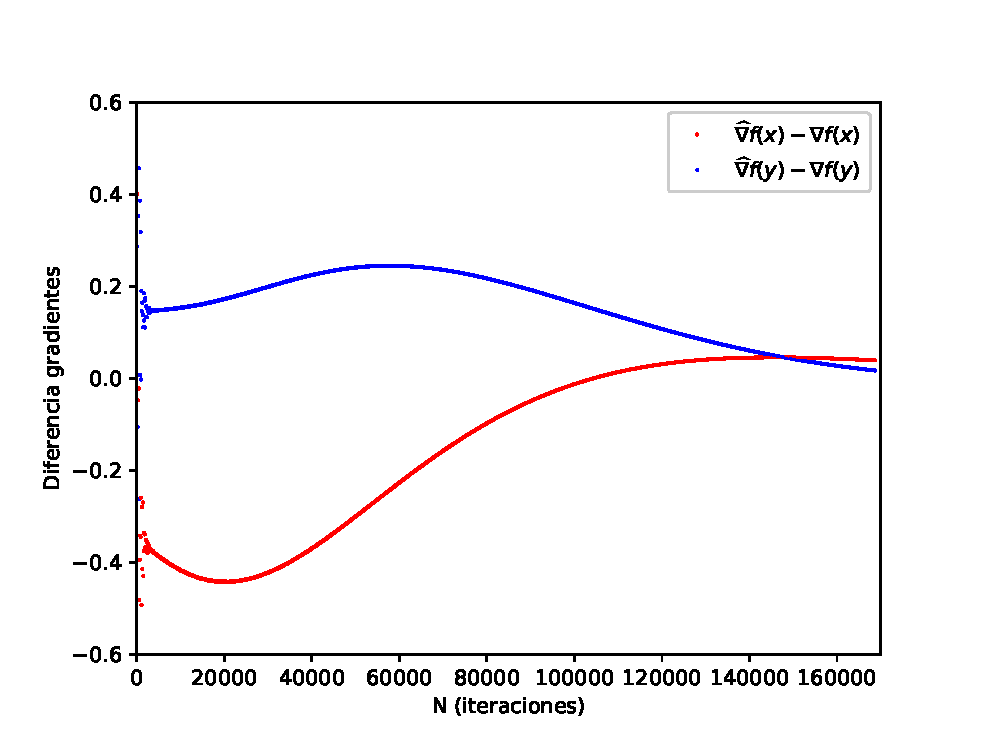
\includegraphics[width=0.75\textwidth]{figures/Graficas_Nuevas/Caso_Inicial/Figure_4.eps}
\caption{Diferencia entre las componentes del gradiente real y el estimado.} \label{Dif_grad}
\end{figure}

\begin{figure}[H]
\centering
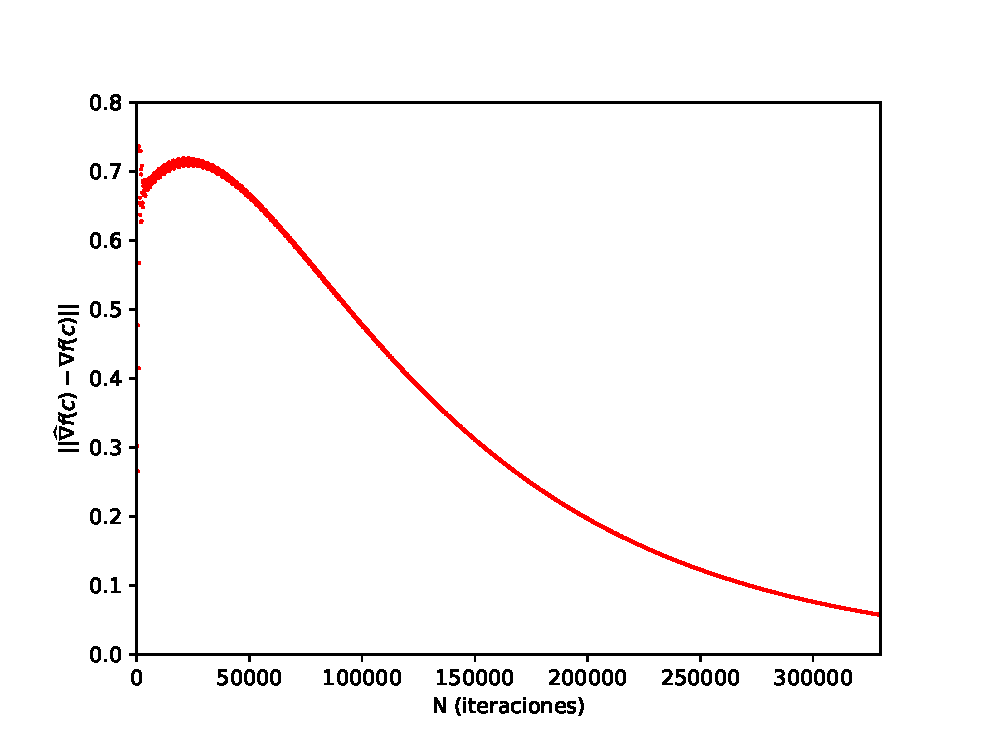
\includegraphics[width=0.75\textwidth]{figures/Graficas_Nuevas/Caso_Inicial/Figure_5.eps}
\caption{Curva de error descrita por la estimación del gradiente.} \label{Curva_error}
\end{figure}

Un comentario destacable es que se deben imponer dos condiciones que necesariamente se deben cumplir para que el algoritmo avance satisfactoriamente. Estas son:

\begin{itemize}
	\item La primera es que el error de formación sea lo más próximo a 0 posible, es decir, que en la medida de lo que cabe los vehículos estarán dispuestos uniformemente en la circunferencia pero con un error que se adicionará al existente por la estima del gradiente. Por ello, se decide imponer que como mucho $e_{\theta}\leq{0.2}$ sobre la ecuación \ref{Error_Coordinacion}.
	\item La segunda consiste en dar una solución satisfactoria para tomar en consideración que ya se ha llegado al punto de interés. Esto se debe a la dificultad de movimiento cuando estés muy cerca del máximo al gradiente hacerse prácticamente 0 y, por lo tanto la formación apenas avanza. Por ello, se impone que para satisfacer condición de máximo, es decir, es solución al problema cuando $f(x)\geq{0.999}$.
\end{itemize}

En la figura \ref{Dif_Caminos} se aprecia como claramente el avance obtenido por el gradiente estimado difiere claramente del real pasando de una recta a definir prácticamente una espiral. Esto era un resultado bastante esperable al acumular un error equiparable al orden 2 de Taylor visto en la ecuación \ref{Fun_Esti}, además se adiciona el error del angulo entre vehículos visto en \ref{Error_Coordinacion} que provocará una estima del gradiente incluso más alejada de lo ideal. Por otro lado, en la figura \ref{grad} se observa la variación de cada componente para cada una de las iteraciones con respecto al gradiente real frente al estimado, una cosa a tener en cuenta es que al inicio se ve como tanto la componente en x como en y del gradiente real empiezan en $cos(45)$ y $sin(45)$ respectivamente y van variando su valor hasta llegar al punto de máxima concentración de sustancias. Este resultado interesa para poder aproximar al error como la diferencia entre ambos, es decir, el resultado mostrado en la figura \ref{Dif_grad}.
\newpage
Recopilando toda esta información y acudiendo a la referencia \cite{Estimacion_Gradiente} el error puede aproximarse como:

\begin{equation} \label{error_gradiente}
	\Delta{\nabla{f\left(c\right)}}=||\hat{\nabla}f\left(c\right)-\nabla{f}\left(c\right)||
\end{equation}

La figura \ref{Curva_error} describe el error dado por la ecuación \ref{error_gradiente}. En este se ve como claramente según se va acercado el conjunto de robots al máximo, el error se va disminuyendo y a la vez que el valor del gradiente tiende a 0 traduciéndose eso en la ecuación \ref{GA} que el avance es menor. Dicha situación se puede aprovechar para evaluar bajo que condiciones el algoritmo funciona mejor, es decir, tal como se describió en la sección \ref{Objetivos_Principales}. Finalmente, es importante evaluar la relación existente entre $\Delta{\nabla{f\left(c\right)}}$ y $\hat{\nabla}{f\left(c\right)}$ con los diferentes parámetros del sistema.

\section{Variación del punto inicial}

\begin{figure}[H]
\centering
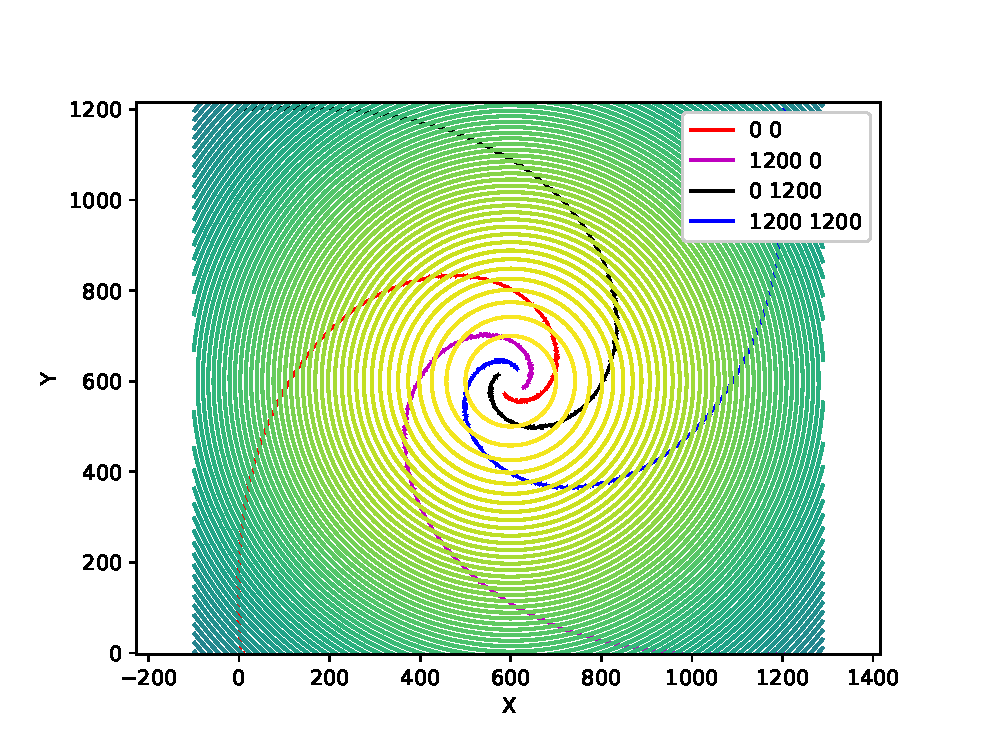
\includegraphics[width=0.70\textwidth]{figures/4_puntos_observar_forma/Figure_1.eps}
\caption{Avance del sistema para diferentes valores de la posición inicial de la formación.} \label{Avance_Posicion}
\end{figure}

La primera situación planteada consiste en utilizar los datos descritos anteriormente\footnote[9]{ N = 4, D = 30 y $\epsilon$=20} para evaluar el efecto que tiene partir desde diferentes puntos. Consecuentemente, se escogen cuatro vértices que forman una diagonal respecto al punto máximo siendo estos $x_o=[0,1200]$, $x_o=[1200,0]$, $x_o=[1200,1200]$ y el origen. El resultado esperable es que la trayectoria descrita posea el mismo punto final \footnote[10]{Máxima concentración de sustancias}, pero lo hará definiendo otra forma, tal como se observo en \ref{Dif_Caminos}. Finalmente, se contempla en la figura \ref{Gradiente_Diversos_Puntos} que las iteraciones persisten para cada punto de partida, por ende el error terminaría siendo similar a \ref{Curva_error} en todos los casos. 

\begin{figure}[H]
  \begin{center}
    \subfigure[Punto 0 0]{
        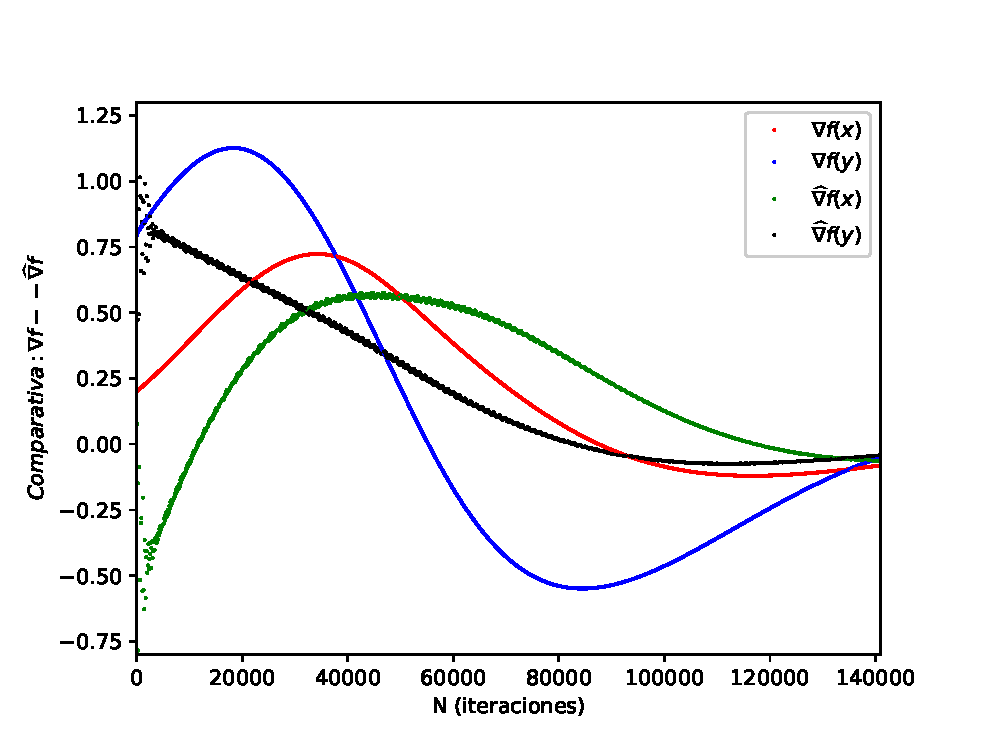
\includegraphics[width=0.45\textwidth]{figures/Graficas_Nuevas/Caso_Inicial/Figure_3.eps}
        }
    \subfigure[Punto 0 1200]{
        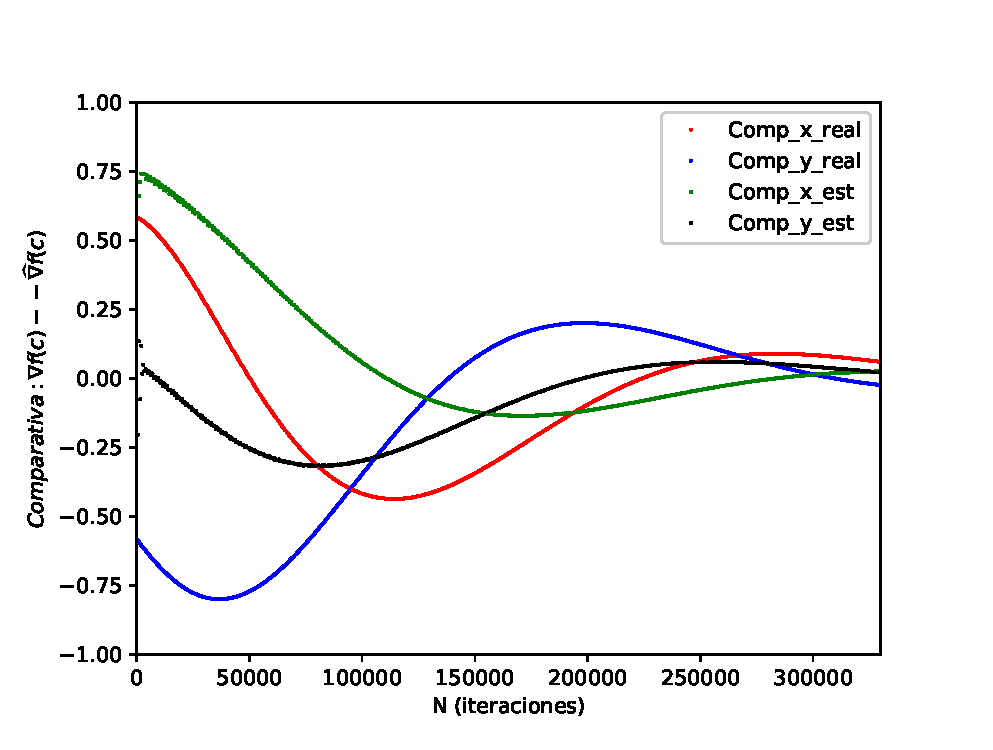
\includegraphics[width=0.45\textwidth]{figures/Graficas_Nuevas/Posicion/0_1200.eps}
        }
	\subfigure[Punto 1200 0]{
        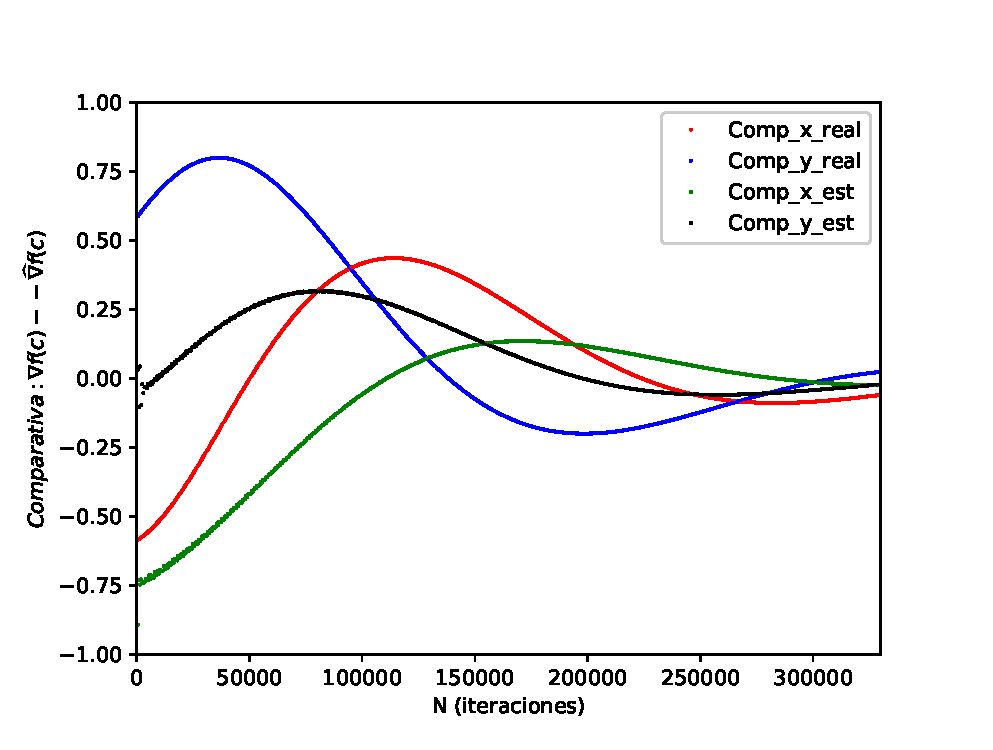
\includegraphics[width=0.45\textwidth]{figures/Graficas_Nuevas/Posicion/1200_0.eps}
        }
	\subfigure[Punto 1200 1200]{
        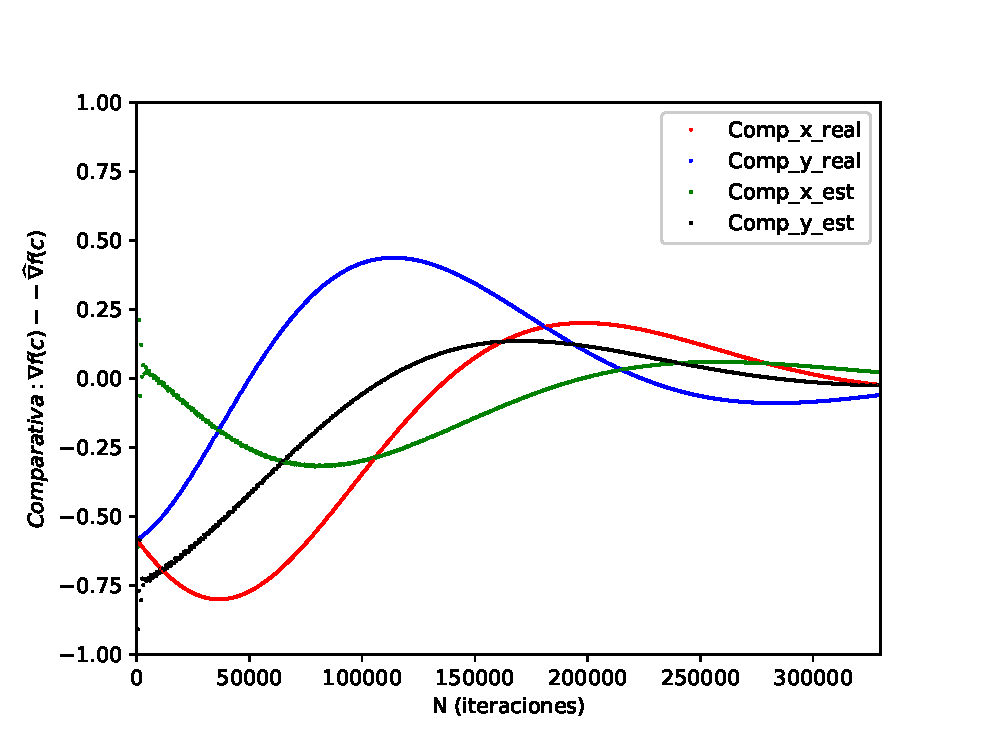
\includegraphics[width=0.45\textwidth]{figures/Graficas_Nuevas/Posicion/1200_1200.eps}
        }
    \caption{Componentes del gradiente estimado y el real para diferentes valores de la posición inicial de la formación.}
    \label{Gradiente_Diversos_Puntos}
  \end{center}
\end{figure}

\section{Variación del número de agentes N}

\begin{figure}[H]
\centering
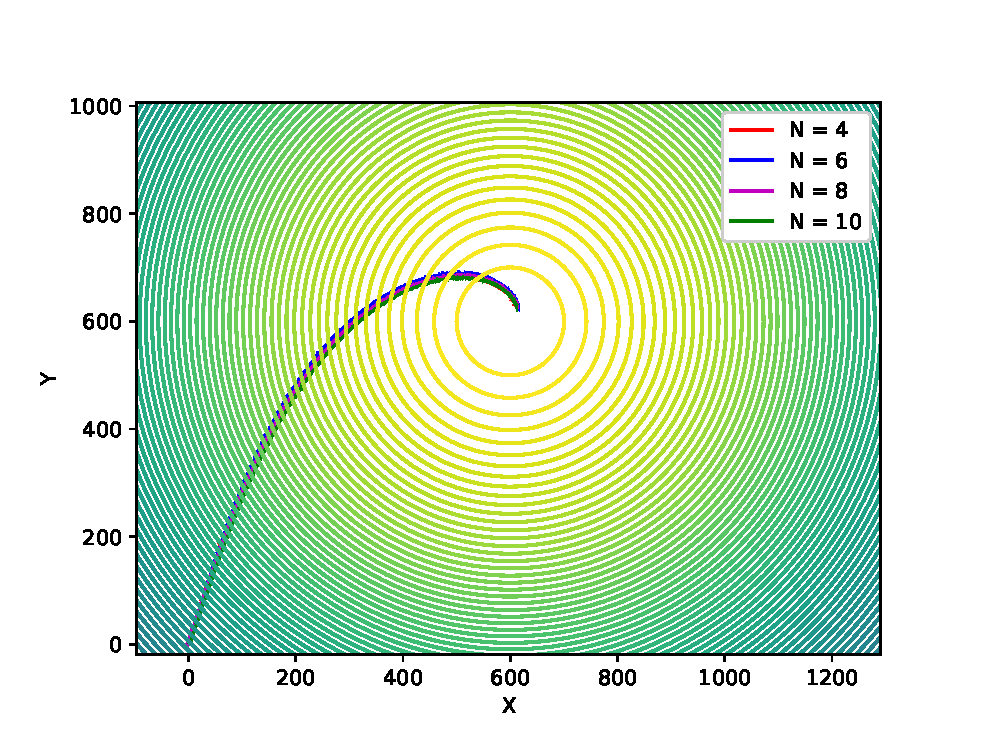
\includegraphics[width=0.70\textwidth]{figures/N_Var_R_50/Figure_1.eps}
\caption{Avance del sistema en función del número de agentes N} \label{N_Var}
\end{figure}

El número de agentes va a influir de dos maneras: 

\begin{enumerate}
	\item Este primer se podía intuir de la gráfica \ref{NAGENTSEST}, en donde claramente se aprecia una dependencia inversamente proporcional, es decir, a medida que se aumenta el número de agentes es de esperarse que el error se reduzca y a su vez las iteraciones necesarias para llegar al máximos se reducen.
	\item No obstante, si se tiene en cuenta el algoritmo de control de formación esto implicaría que cada vez tu número de agentes va creciendo teniendo más nodos dentro del sistema y por ello se ha de pasar mucha más información al presentar mas nodos adyacentes. A esto se le añade el tiempo que se tendría que esperar para que los N vehículos se dispongan de uniformemente en la formación.
\end{enumerate}

Se puede apreciar como la trayectoria descrita en \ref{N_Var} no cambia significativamente. Sin embargo, si tiene un impacto en el número de iteraciones \ref{Gradiente_N_Var} y en la reducción del error \ref{N_Var_Error}. Para este último caso, se tiene que a partir de un determinado número de agentes el sistema se vuelve invariante, es decir, existe un valor de N límite para la reducción del error.

\begin{figure}[H]
  \begin{center}
    \subfigure[N = 4]{
        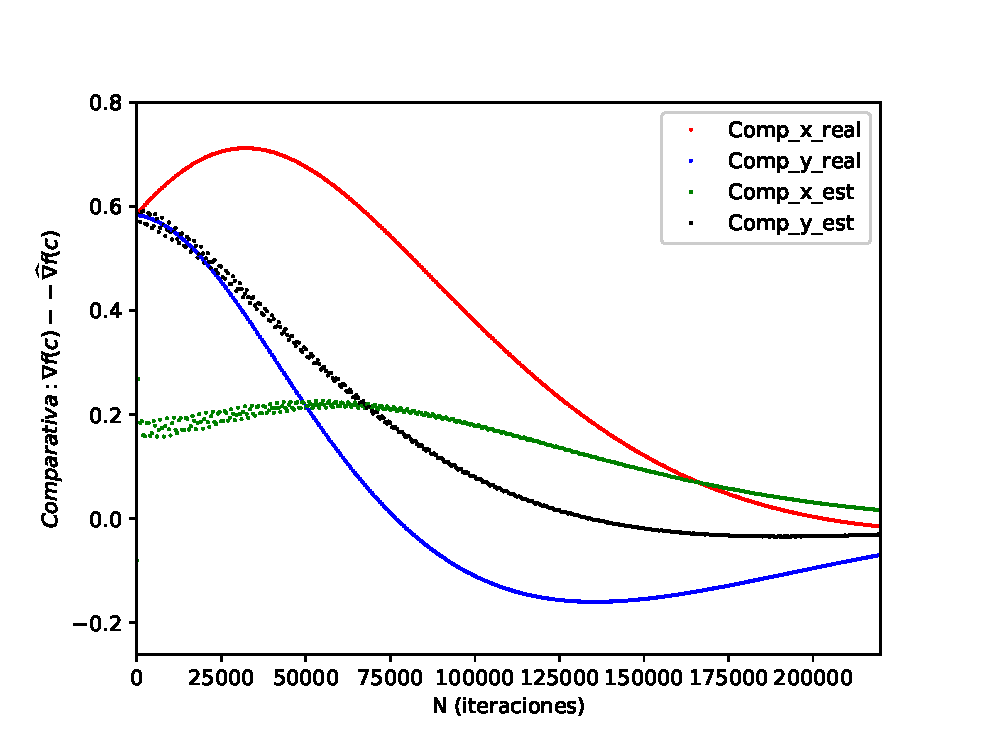
\includegraphics[width=0.45\textwidth]{figures/Graficas_Nuevas/N/N4.eps}
        }
    \subfigure[N = 6]{
        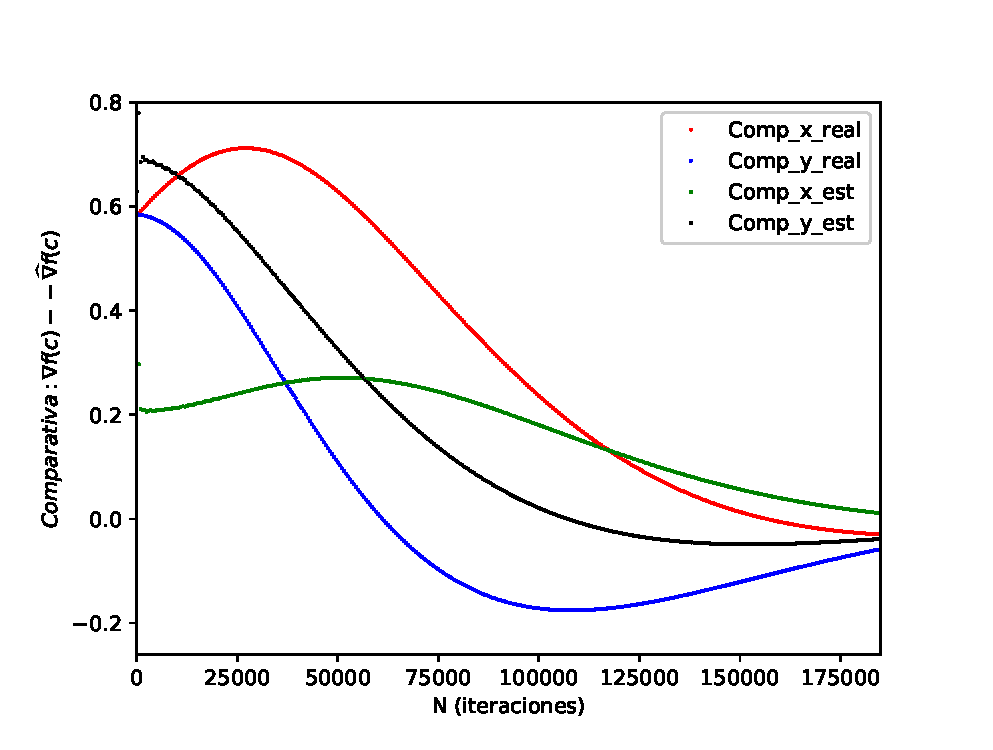
\includegraphics[width=0.45\textwidth]{figures/Graficas_Nuevas/N/N6.eps}
        }
	\subfigure[N = 8]{
        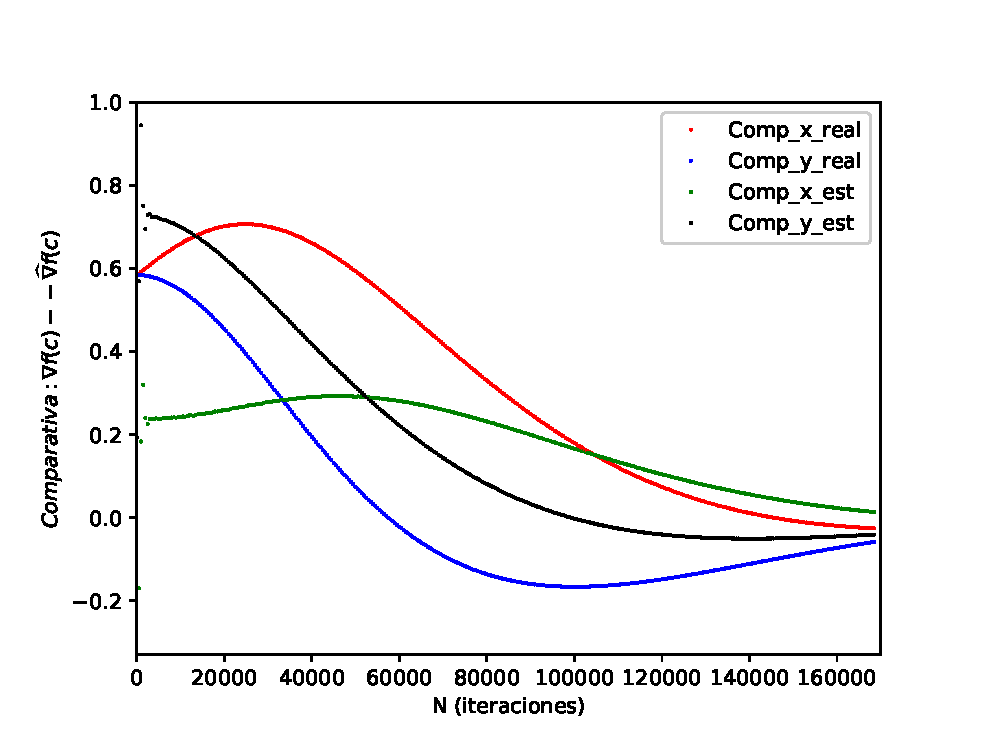
\includegraphics[width=0.45\textwidth]{figures/Graficas_Nuevas/N/N8.eps}
        }
	\subfigure[N = 10]{
        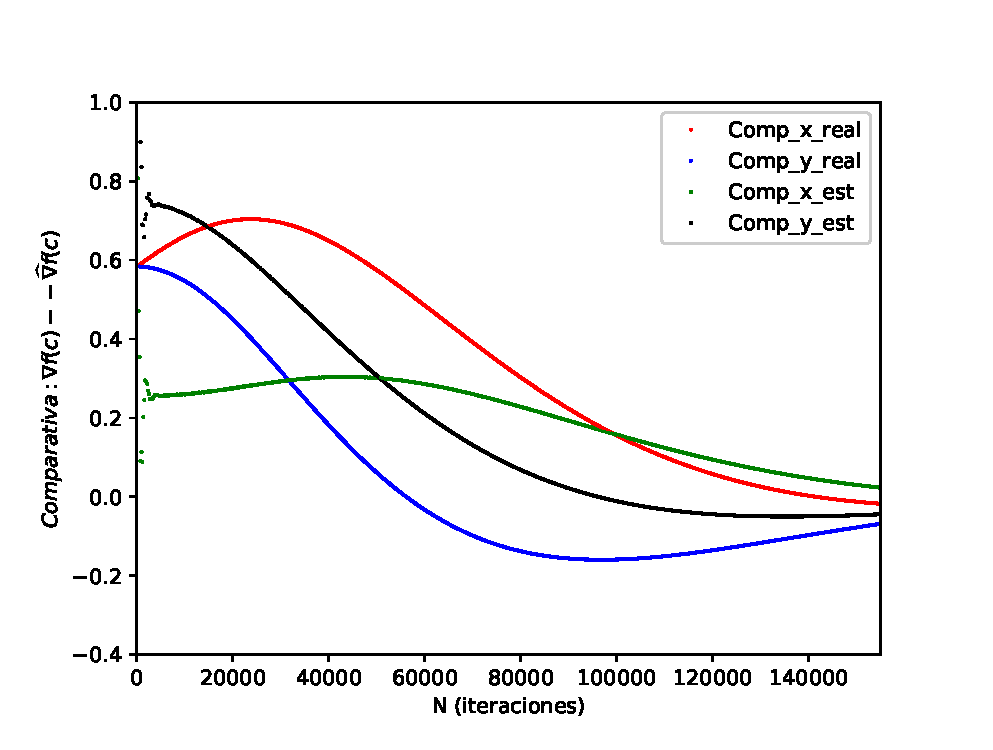
\includegraphics[width=0.45\textwidth]{figures/Graficas_Nuevas/N/N10.eps}
        }
    \caption{Evaluación de las componentes del gradiente estimado y el real en función del número de agentes N.}
    \label{Gradiente_N_Var}
  \end{center}
\end{figure}

Adicionalmente, se aprecia que el valor de ambas componentes del gradiente va a oscilar cuando el valor de la función no es próximo a 1 y el número de agentes es relativamente pequeño.

\begin{figure}[H]
\centering
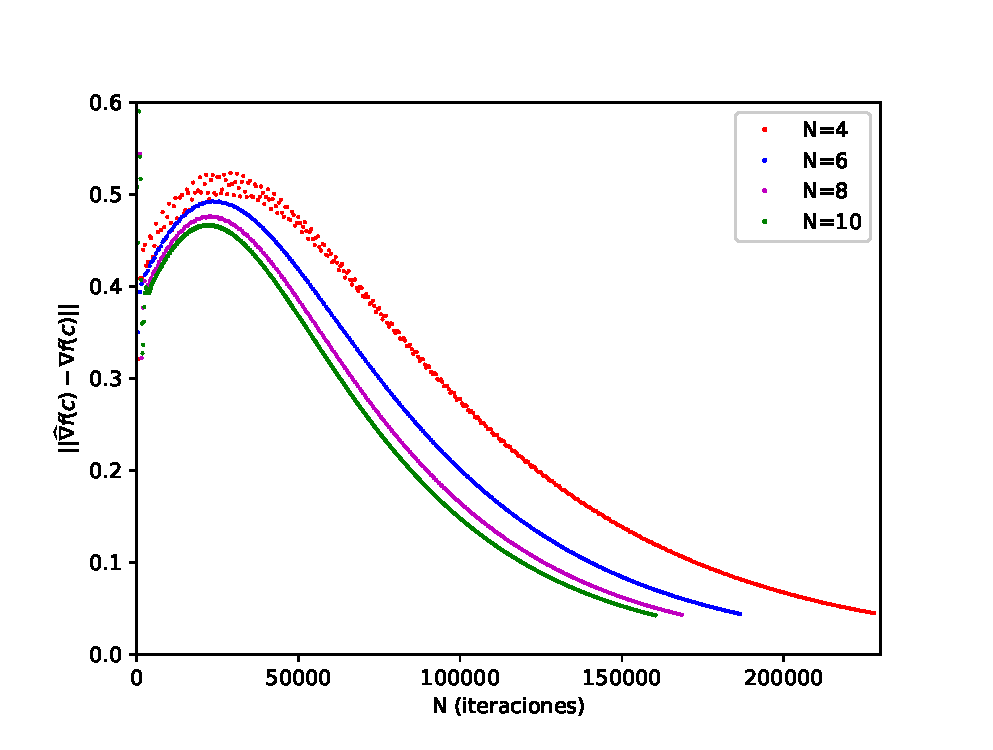
\includegraphics[width=0.70\textwidth]{figures/Graficas_Nuevas/N/Figure_5.eps}
\caption{Error descrito por el gradiente esrimado al variar el número de agentes N.} \label{N_Var_Error}
\end{figure}

\section{Variación del radio D}

\begin{figure}[H]
\centering
\includegraphics[width=0.70\textwidth]{figures/Dif_R_BU/Figure_1.eps}
\caption{Avance del sistema en función del radio D.} \label{D_Var}
\end{figure}

Imponiendo que N = 4 y $\epsilon$=20, se evalúa la influencia del radio D. Se aprecia que el sistema en sí es mucho más sensible al radio de la formación que al número de agentes. Si retomas la referencia \cite{Adicional_Estimacion_1} acota al error de la siguiente forma:
\begin{equation}\label{Depe}
	||\hat{\nabla}f\left(c\right)-\nabla{f}\left(c\right)||\leqslant{D·L}
\end{equation}

En donde, $L$ es un escalar delimitado por el error de la serie de Taylor original. Si bien es cierto que el error depende del radio de la formación D de tal forma que un aumento conlleva a tener más error al darle mayor margen sobre la desigualdad \ref{Depe}.

\begin{figure}[H]
  \begin{center}
    \subfigure[D = 30]{
        \includegraphics[width=0.45\textwidth]{figures/Graficas_Nuevas/D/D30.eps}
        }
    \subfigure[D = 40]{
        \includegraphics[width=0.45\textwidth]{figures/Graficas_Nuevas/D/D40.eps}
        }
	\subfigure[D = 50]{
        \includegraphics[width=0.45\textwidth]{figures/Graficas_Nuevas/D/D50.eps}
        }
	\subfigure[D = 60]{
        \includegraphics[width=0.45\textwidth]{figures/Graficas_Nuevas/D/D60.eps}
        }
    \caption{Evaluación de la componentes del gradiente estimado y el real en función del radio D.}
    \label{Gradiente_Var_D}
  \end{center}
\end{figure}

En la formación de control va a influir directamente el radio de la circunferencia dado que entre mayor sea D el error prefijado será menos restrictivo y por ende aprecias comportamientos oscilantes en las zonas lejanas al máximo de radiación.

Evaluando únicamente al radio D se ve como a medida que su valor decrece el error aumenta y con ello el número de iteraciones de una forma mucho más notoria que el número de agentes. 

\begin{figure}[H]
\centering
\includegraphics[width=0.70\textwidth]{figures/Graficas_Nuevas/D/DVariable.eps}
\caption{Error descrito por el gradiente estimado al variar el radio D.} \label{D_Var_Error}
\end{figure}

\section{Variación del peso $\epsilon$}

Este caso va a estar estrictamente relacionado con \ref{GA} dado que si se aumenta el valor de $\epsilon$ es de esperarse que la formación más en la dirección del gradiente y uno se plantea que posiblemente llegue más rápido al punto máximo. No obstante, al aumentar el peso que multiplica al gradiente a su vez estas arrastrando al error provocando que la trayectoria descrita por la espiral se acentué mucho más. Este efecto es apreciable en la \ref{Epsilon_Var}.

\begin{figure}[H]
\centering
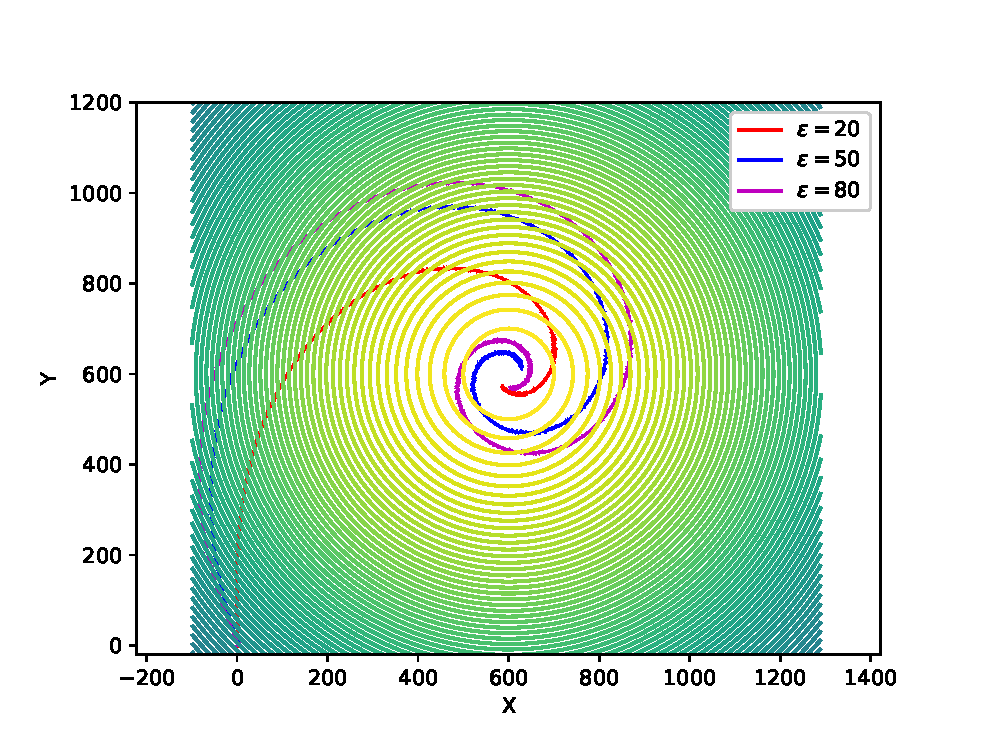
\includegraphics[width=0.72\textwidth]{figures/Epsilon_variante/Figure_1.eps}
\caption{Avance del sistema en función del radio peso $\epsilon$.} \label{Epsilon_Var}
\end{figure}

\begin{figure}[H]
\centering
\includegraphics[width=0.72\textwidth]{figures/Graficas_Nuevas/E/EPSILONVAR2.eps}
\caption{Error descrito por el gradiente estimado al variar el peso $\epsilon$.} \label{Epsilon_Var_Error}
\end{figure}

El comportamiento del peso $\epsilon$ esta claramente diferido su efecto sobre el gradiente estimado y sobre el gradiente real, en el primero de estos es apreciable  en la figura \ref{Epsilon_Var_Error} que aumentarlo es perjudicial para el algoritmo dado que conllevaría a elevar en exceso tanto el número de iteraciones como $\Delta{\nabla{f\left(c\right)}}$. Este efecto era justo el contrario con el gradiente real, en donde si aumentas el valor de dicho peso se daban casos donde llegabas con menos pasos al máximo.

\begin{figure}[H]
  \begin{center}
    \subfigure[$\epsilon$ = 20]{
        \includegraphics[width=0.41\textwidth]{figures/Graficas_Nuevas/E/E20.eps}
        }
    \subfigure[$\epsilon$ = 50]{
        \includegraphics[width=0.41\textwidth]{figures/Graficas_Nuevas/E/E50.eps}
        }
	\subfigure[$\epsilon$ = 80]{
        \includegraphics[width=0.41\textwidth]{figures/Graficas_Nuevas/E/E80.eps}
        }
    \caption{Evaluación de las componentes del gradiente estimado y el real en función del peso $\epsilon$.}
    \label{Gradiente_Var_Epsilon}
  \end{center}
\end{figure}

Finalmente, se procederá a evaluar un caso particular en el que se tienen múltiples fuentes emitiendo con el objetivo de demostrar las limitaciones que presenta la utilización del algoritmo de ascenso de gradiente.

\section{Evaluación con múltiples fuentes}

En este caso se va a considerar que N = 4, D = 50 y $\epsilon$=20, además el nuevo plano sobre el que se desplaza el enjambre se describe según:

\begin{itemize}
	\item Una primera gaussiana con los siguientes datos: el centro se situé en $c_{o}=[0,1200]$, un ángulo $\theta=0$ , una desviación uniforme en ambos ejes $\sigma_{x}=\sigma_{y}=\frac{1}{300}$ para que la matriz quede definida como $S = \bigl[\begin{smallmatrix}\frac{300}{\sqrt{2}} & 0\\ 0 & \frac{300}{\sqrt{2}}\end{smallmatrix}\bigr]$  y cuyo volumen es $p = 0.9$. 
	\item Una segunda gaussiana con los siguientes datos: el centro se situé en $c_{o}=[1200,0]$, un ángulo $\theta=0$ , una desviación uniforme en ambos ejes $\sigma_{x}=\sigma_{y}=\frac{1}{300}$ para que la matriz quede definida como $S = \bigl[\begin{smallmatrix}\frac{300}{\sqrt{2}} & 0\\ 0 & \frac{300}{\sqrt{2}}\end{smallmatrix}\bigr]$  y cuyo volumen es $p = 0.9$.
	\item Una segunda gaussiana con los siguientes datos: el centro se situé en $c_{o}=[0,1200]$, un ángulo $\theta=\frac{\pi}{6}$ , una desviación distinta en cada eje con $\sigma_{x}=\frac{1}{1000}$ y $\sigma_{y}=\frac{1}{500}$  para que la matriz quede definida como $S = \bigl[\begin{smallmatrix}\frac{1000}{\sqrt{2}} & 0\\ 0 & \frac{500}{\sqrt{2}}\end{smallmatrix}\bigr]$ y cuyo volumen es $p = 1$. 
\end{itemize}

Todos estos datos referidos a lo visto en la sección \ref{Simulacion_Modelo}. Al sumarlas se obtiene:

\begin{figure}[H]
  \begin{center}
    \subfigure[Vista en 3D]{
        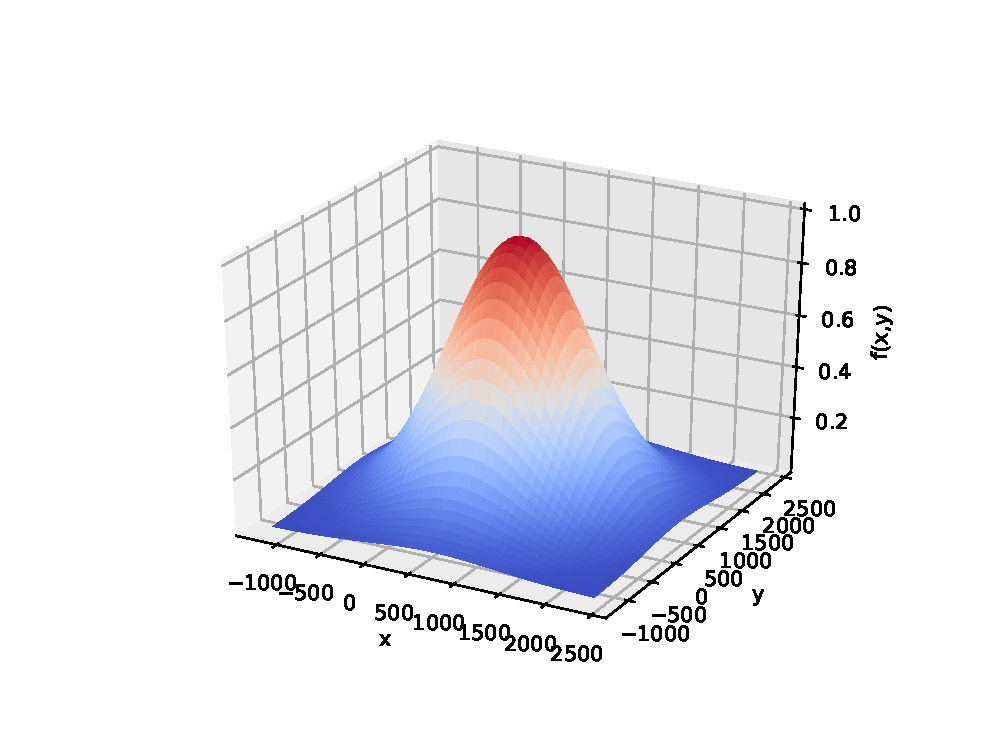
\includegraphics[width=0.45\textwidth]{figures/Casos_Especiales/Gaussiana.eps}
        }
    \subfigure[Curvas de nivel]{
        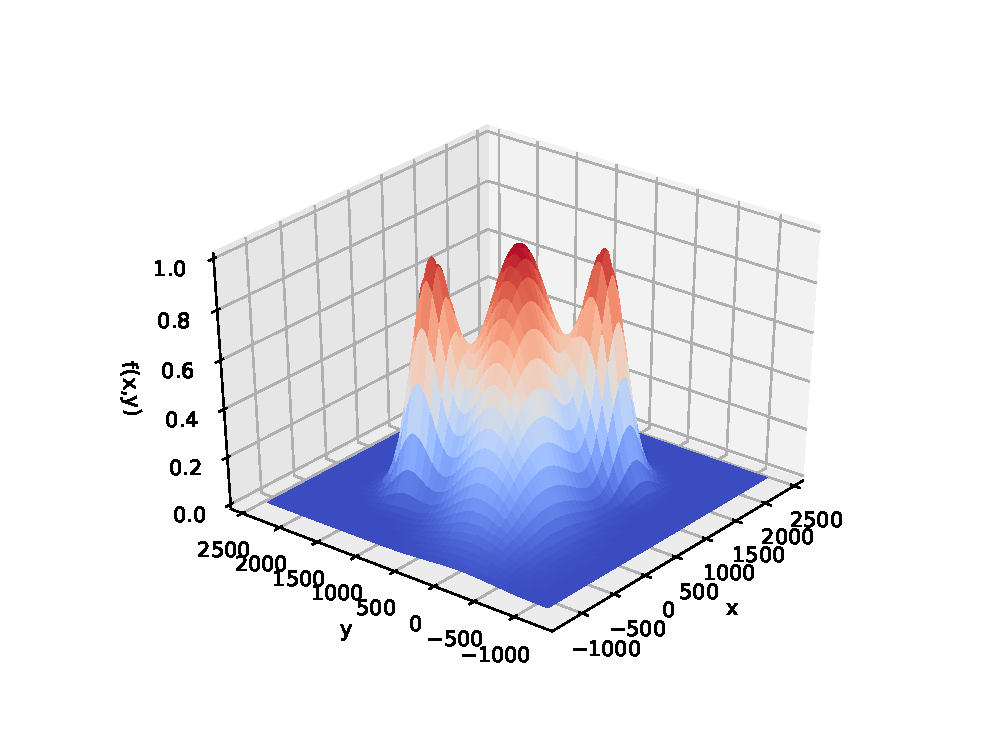
\includegraphics[width=0.45\textwidth]{figures/Casos_Especiales/Gaussiana_meh.eps}
        }
    \caption{Resultado de sumar las tres funciones gaussianas. Nuevo modelo para la simulación.}
    \label{New_Gaussiana}
  \end{center}
\end{figure}
\newpage
Con esta nueva función surgen dos casos de interés:

\begin{enumerate}
	\item El primero es que se tienen múltiples máximos, en concreto, dos locales y el global. Por lo que puede suceder que dependiendo del número de agentes N, el radio D o el peso $\epsilon$ vaya hacia cualquiera de los tres. Sin embargo, como ya se hizo un estudio para cada uno de ellos directamente se evalúan las posiciones de partida del enjambre para observar hacia que fuente de emisión se dirige.
	\item El segundo son los puntos silla generados entre los tres máximos. Estos haciendo uso del gradiente real conformaban un problema al utilizar el algoritmo de ascenso de gradiente al hacerse $\nabla{f\left(c\right)}=0$. No obstante, se verá que en este caso eso no va a suceder.
\end{enumerate}
	
\begin{figure}[H]
\centering
\includegraphics[width=0.75\textwidth]{figures/Multi_Gaussiana/Figure_1.eps}
\caption{Avance definido sobre el plano con múltiples fuentes en tres puntos diferentes} \label{Multiples_Fuentes}
\end{figure}

\begin{figure}[H]
  \begin{center}
    \subfigure[$f\left(x\right)=0.999$]{
        \includegraphics[width=0.45\textwidth]{figures/Graficas_Nuevas/Multi/00MULTI.eps}
        }
    \subfigure[$f\left(x\right)=0.970$]{
        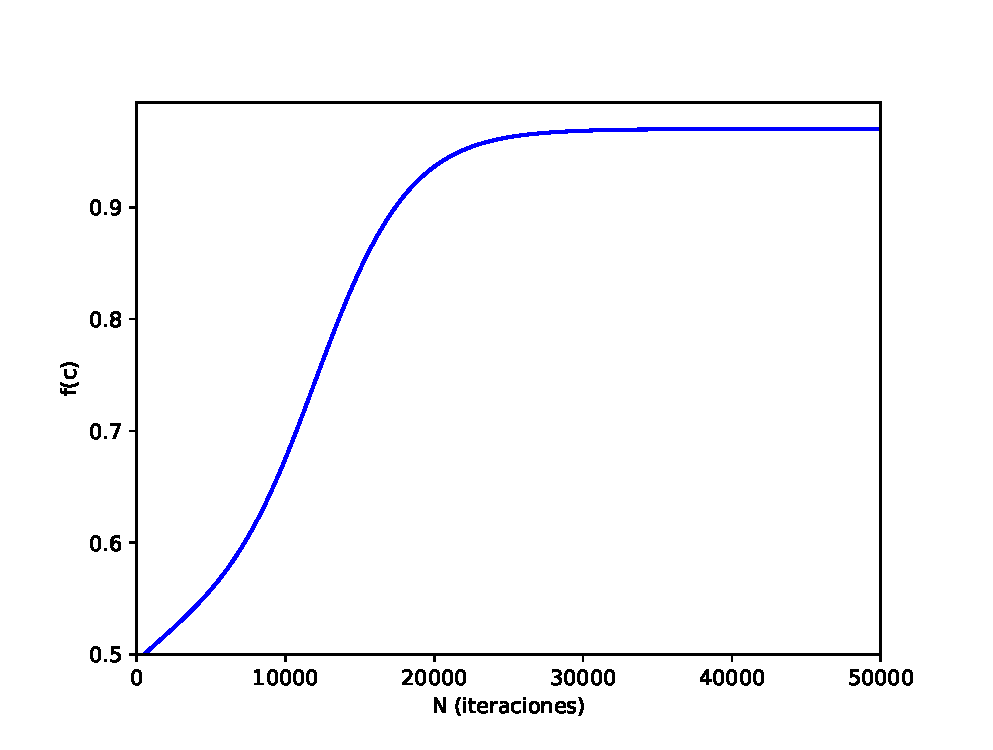
\includegraphics[width=0.45\textwidth]{figures/Graficas_Nuevas/Multi/f_99.eps}
        }
    \caption{Comparación del valor máximo de ambas fuentes}
    \label{Fun_Gauss_Multi}
  \end{center}
\end{figure}

Comparando los valores obtenidos para los caminos azul y rojo de \ref{Multiples_Fuentes} a partir de la figura \ref{Fun_Gauss_Multi}, se observa como dados dos posiciones iniciales el algoritmo no es capaz de distinguir cual de los dos es el que posee mayor concentración de sustancias. Esto se debe a una limitación del propio algoritmo el cual únicamente te va a estar continuamente elevando el valor de la función hasta encontrar un máximo más no tendrá la capacidad de distinguirlos.

\begin{figure}[H]
  \begin{center}
    \subfigure[Inicio en 0 0]{
        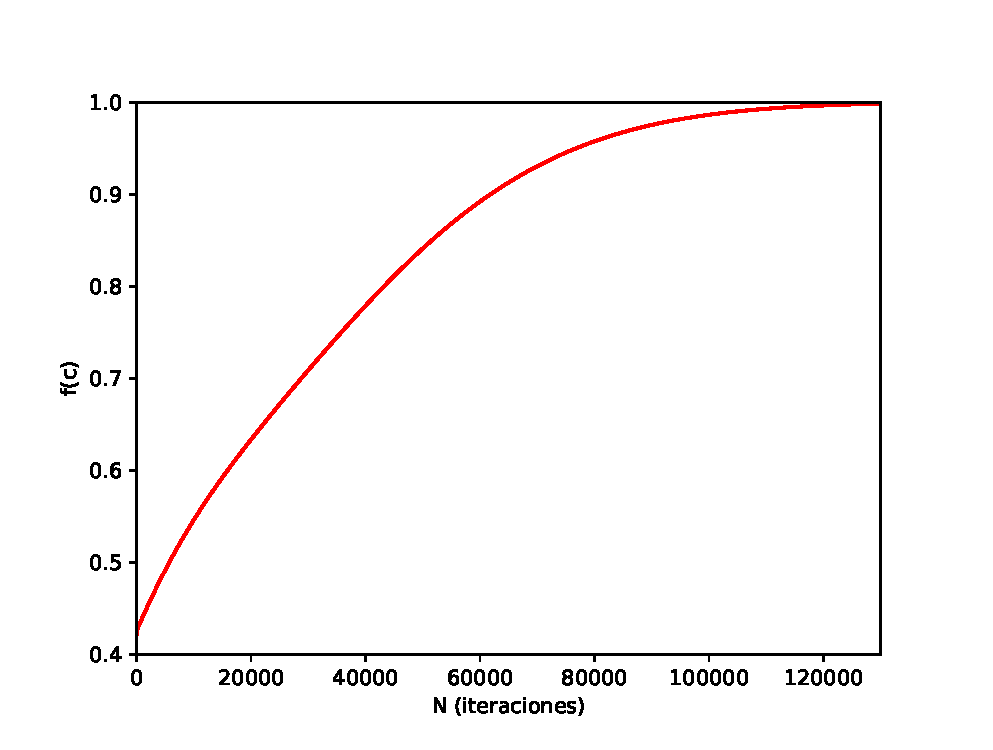
\includegraphics[width=0.45\textwidth]{figures/Graficas_Nuevas/Multi/FC.eps}
        }
    \subfigure[Inicio en 0 800]{
        \includegraphics[width=0.45\textwidth]{figures/Graficas_Nuevas/Multi/Fun_3.eps}
        }
    \caption{Evaluación de las componentes del gradiente estimado según la fuente objetivo y el punto de partida}
    \label{Comp_Multi_Gaussian}
  \end{center}
\end{figure}

Una segunda cosa que surge de recorrer los máximos locales es que se encuentran definidos de forma plana en el centro \footnote[11]{El valor del gradiente es casi nulo}, y por ende el avance por dicha zona va a ser prácticamente imposible que el sistema avance. Esto se refleja si se observan las componentes del gradiente estimado en la figura \ref{Comp_Multi_Gaussian} estas conforman una recta horizontal que no esta exactamente en cero pero tiende hacia dicho valor, es decir, esta acotada. Otro aspecto que se aprecia es el grosor de las componentes y esto se puede asociar al error, traduciéndose en que si la estima del gradiente posee un error muy pronunciado el sistema tenderá a presentar oscilaciones.

Por otro lado, la trayectoria de color rosa en \ref{Multiples_Fuentes} consistía en definir una situación inicial que se encuentre justo sobre el punto silla. En el caso de utilizar el gradiente estimado esto no va a suponer un problema al tener el gradiente un error, en este caso dicho error va a representar una ventaja dado que permite al algoritmo salirse de ese tipo de situaciones, es decir, los puntos sillas pasan desapercibidos gracias a la operación conjunta de los tres algoritmos.

Finalmente, todas las simulaciones obtenidas a lo largo de este capitulo se basaron en \cite{Git_Hector}, el cual contiene el algoritmo de coordinación original y \cite{Git_todos} contiene las modificaciones necesarias para que los tres algoritmos funcionen en conjunto.





